\documentclass{article}
\usepackage{graphicx}
\usepackage{hyperref}
\usepackage{caption}
\usepackage{subcaption}
\usepackage{mathtools}
\usepackage[dutch]{babel}

\begin{document}

\begin{center}
	\huge{Wiskunde in Kunst}\\
	\LARGE{Opdracht 9} \\
	
	\vspace{2cm}
	
	\Large{De Gulden snede}\\
	
	\vfill
	
	\begin{figure}[Hh]
		\centering
		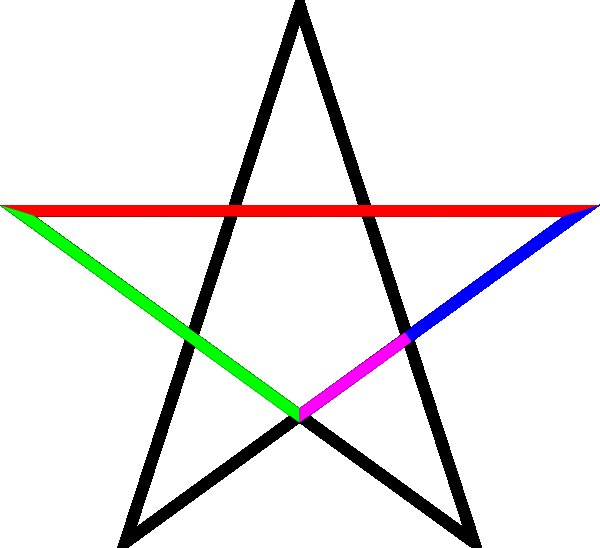
\includegraphics[width=\textwidth]{Pentagram-phi.jpg}
	\end{figure}
	
	\vfill
	\Large{Marcelo Dias Avelino} \hfill \large{0840416}
\end{center}

\thispagestyle{empty} % Remove page numbering

\pagebreak

\setcounter{page}{1} % Start counting pages here

\section{De gulden snede}

De gulden snede is een bekende verhouding in de wiskunde. Het houdt in dat bij twee lengtes, de verhouding tussen hun optelling en de grootste waarde gelijk is aan de verhouding tussen beide lijnen, zoals afgebeeld in Figuur \ref{fig:ratio-lines}. In dit geval is de verhouding tussen \( \frac{a+b}{a} \) gelijk aan \( \frac{a}{b} \). Dit verhouding wordt aangegeven met de griekse letter \(\varphi\) (phi) en staat gelijk aan \(\varphi = \frac{1+\sqrt{5}}{2} \approx 1.6180339887\). 

\begin{figure}[Hh]
	\centering
	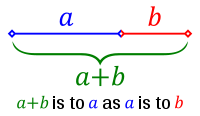
\includegraphics[width=0.35\textwidth]{golden-ratio-line.png}
	\caption{De verhouding tussen twee lengtes.}
	\label{fig:ratio-lines}
\end{figure}

De wiskundige eigenschappen van dit getal worden als sinds de oudheid bestudeerd, maar het heeft de term \textit{gulden snede} pas in de 19e eeuw gekregen. Het vroegst bekende studie van dit getal stemt uit de tijd van Oude Griekland. De grieken waren begonnen met het bestuderen van de gulden snede vanwege zijn regelmatig verschijning in de geometrie en zijn een belangrijkheid om pentagrammen en pentagonnen te tekenen. De griekse wiskundig Euclides heeft in zijn meetkundig en rekenkundig verzamelwerk, de \textit{Elementen}, de eerste bekende definitie van wat nu bekend staat als de gulden sneden. Euclides beschreef het als ``Een rechte lijn is zogenaamd gesneden in de extreme en gemiddelde verhouding wanneer, zoals het gehele lijn staat voor de grootste segment, zo staat de grotere tot de kleinere.''. Door het gehele boek wordt de gulden snede gebruikt bij meerdere stellingen en hun bewijs. De verhouding was verder onderzocht in het boek \textit{De divina proportione} (De goddelijke properties) van de italianse wiskundig Fra Luca Bartolomeo de Pacioli, een mede-collaborateur van Leonardo da Vinci en een van de oorspronkelijk bijdragers aan het vakgebied van accountancy. Dit boek beschrijft de gulden snede vanuit een wiskundig inkijk hoek en bestudeert ook polygonen, een figuur in een plat vlak gevormd door rechte lijnen. Sinds de 20e eeuw is de gulden snede gepresenteerd door de letter \(\varphi\), genoemd naar de griekse beeldhouwer Phidias, die de gulden snede gebruikte in zijn kunst. Het wordt ook gepresenteerd door de letter \(\tau\) (tau), die `snijden' betekent.

\section{Gebouwen}

De guldens snede kun je overal tegenkomen. Het is te vinden in de verhoudingen van gebouwen, verhoudingen van gezicht, verhoudingen van bloemen, etc.. Er zijn mensen die geloven dat het begrip van schoonheid heel nauw met \(\varphi\) samenhangt. Bekende gebouwen die ontworpen zijn met de gulden snede als basis zijn bijvoorbeld de grote piramide van Giza of het Parthenon in Athene. 

In Figuur \ref{fig:parthenon} is de gulden snede te zien in het ontwerp van de Parthenon. Op de afbeelding is de spiraal van Fibonacci over de Parthenon getekend. Dit spiraal is gebaseerd op de Fibonacci reeks, een reeks die onstaat door de vorige twee getallen met elkaar op te tellen. De verhouding tussen elke getal en zijn voorgaande getal komt uit heel erg in de buurt van de gulden snede uit. Door deze spiraal over de Parthenon te tekenen is het makkelijk om gulden snede bij elke onderdeel terug te zien komen, bijvoorbeld de bovenkant van de zuilen en de base van de daklijn zijn in gulden snede proporties tot de hoogte van het gebouw. Verder is er in Figuur \ref{fig:parthenon-columns} de verhoudingen van de Parthenon in meer detaille te zien. De draagbalk op de zuilen is in gulden snede verhouding met de zuilen zelf. Ook heeft de draagbalk een lijn die het verdeelt in twee soorten decoraties. Deze twee gedeeltes zijn ook in de juiste verhouding met elkaar. Verder is de breedte van de zuilen ook in verhouding met de ruimte tussen de zuilen samen met de breedte van de volgende zuil. Maar de mooiste en duidelijkst voorbeeld van de \(\varphi\) verhouding in dit gebouw is te vinden in de draagbalk zelf. In Figuur \ref{fig:parthenon-beam} is de Fibonacci spiraal weer te zien, maar deze keer overlapt over de versieringen. In de afstanden en lengtes van alle componenten van de versieringen op de draagbalk is het duidelijk te zien dat de grieken heel goed hebben nagedacht over elke detaille en dat ze zeker bekend waren met de gulden snede.

\begin{figure}[Hh]
    \centering
    \begin{subfigure}[b]{0.55\textwidth}
        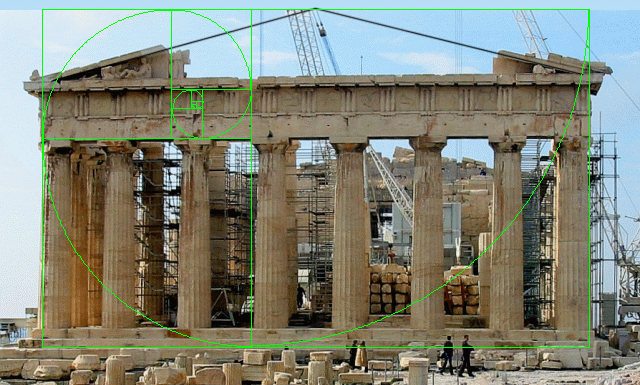
\includegraphics[width=\textwidth]{parthenon.png}
		\caption{De parthenon met de Fibonacci spiraal.}
		\label{fig:parthenon}
    \end{subfigure}
    ~ 
    \begin{subfigure}[b]{0.3\textwidth}
        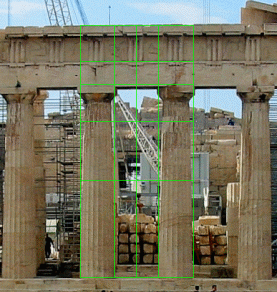
\includegraphics[width=\textwidth]{parthenon-columns.png}
		\caption{De proporties van de zuilen.}
		\label{fig:parthenon-columns}
    \end{subfigure}%
    ~
	\begin{subfigure}[b]{0.45\textwidth}
        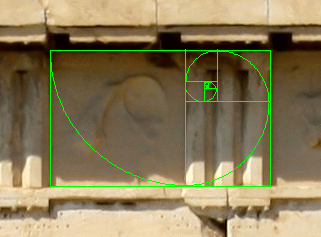
\includegraphics[width=\textwidth]{parthenon-beam.png}
		\caption{De proporties van de draagbalk.}
		\label{fig:parthenon-beam}
    \end{subfigure}%
    
    \caption{De gulden snede in de Parthenon.}
    \label{fig:parthenon-phi}
\end{figure}

De grote piramide van Giza is gebaseerd op phi op een andere manier. Er is veel bewijs dat de piramide gebaseerd is op drie verschillende wiskundige bases: Phi, de gulden snede, Pi, de relatie van de omtrek van een cirkel tot zijn diameter, en de stelling van Pythagoras, de stelling gebruikt om de lengte van een zijn van een driehoek uit te rekenen mits de lengtes van de 2 resterende zijdes bekend zijn. Phi is de enige getal waarbij zijn kwadraat gelijk is aan phi plus \'e\'en, ofwel \(\varphi + 1 = \varphi^2\) of \(1.618 + 1 = 2.168\). Door deze vergelijking te gebruiken is het mogelijk om een zogenaamd \textit{gulden driehoek} te construeren. Dit is een driehoek met de lengtes \(\sqrt{\varphi}\), \(\varphi\) en 1, zoals afgebeeld in Figuur \ref{fig:driehoek}. Hierdoor ontstaat een piramide met een breedte van 2 driehoeken breed, een hoogte van \(\sqrt{\varphi} = 1.272\) waarbij de verhouding tussen bodem en top \(\frac{1.272}{2} = 0.636\) is. Als dit vergeleken wordt met de afmetingen van de piramide van Giza, ofwel 230.4 meters breed en 146.5 meter hoog, komen we achter dat het gebaseerd is op de gulden driehoek (\(\frac{146.5}{230.4} = 0.636\)).

\begin{figure}[Hh]
    \centering
	\begin{subfigure}[b]{0.5\textwidth}
        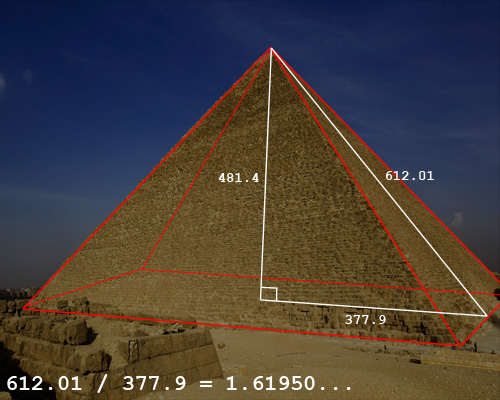
\includegraphics[width=\textwidth]{pyramid.jpg}
        \caption{De grote piramide van Giza.}
        \label{fig:giza}
    \end{subfigure} %
    ~
    \begin{subfigure}[b]{0.3\textwidth}
        \includegraphics[width=\textwidth]{Golden-Triangle-Pythagorus.png}
        \caption{De gulden driehoek.}
        \label{fig:driehoek}
    \end{subfigure}
    \caption{De gulden snede in de grote pyramid van Giza.}
    \label{fig:pyramid-phi}
\end{figure}

\section{Natuur}

De mens is niet de enige die gebruik maakt van de gulden snede, deze verhouding komt heel vaak voor in de natuur. Een voorbeeld ervan is de positionering van en het aantal zaden in een zonnebloem. Zoals het te zien valt in Figuur \ref{fig:sunflower}, zijn de zaden gepositioneerd volgens de spiraal van Fibonacci. Verder valt het aantal zaden ook binnen de Fibonacci reeks, er kunnen zelfs zoveel als 144 zaden aanwezig zijn in \'e\'en bloem. Een andere voorbeeld van de phi verhouding in de natuur zijn de aantal taken in een boom of het aantal bladeren in een taak. In Figuur \ref{fig:tree} is een manier afgebeeld hoe de taken van een boom verdeeld kunnen zijn over het helemaal en volgens de Fibonacci reeks. Maar misschien het bekendst en duidelijkste voorbeeld dat te vinden is in de natuur is de schelp van een soort inktvis genaamd nautilus. De schelp van deze is een perfecte match van de spiraal van Fibonacci.

\begin{figure}[Hh]
    \centering
    \begin{subfigure}[b]{0.48\textwidth}
        \includegraphics[width=\textwidth]{sunflower.jpg}
		\caption{De zaden van een zonnebloem.}
		\label{fig:sunflower}
        
        \includegraphics[width=\textwidth]{tree.jpg}
		\caption{De taken van een boom.}
   		\label{fig:tree}
    \end{subfigure}
	~ % 
    \begin{subfigure}[b]{0.48\textwidth}
        \includegraphics[width=\textwidth]{nautilus.jpg}
		\caption{De schelp van een nautilus.}
		\label{fig:nautilus}
    \end{subfigure}
    
    \caption{De gulden snede in de natuur.}
    \label{fig:nature-phi}
\end{figure}

\end{document}